\documentclass[12pt]{caltech_thesis}
\usepackage[hyphens]{url}
\usepackage{graphicx}
\usepackage[romanian]{babel}
\usepackage{todonotes}
\usepackage{mathtools}
\usepackage{amsmath}

\usepackage[utf8]{inputenc}
\usepackage[T1]{fontenc}
\usepackage{newtxtext,newtxmath}

\usepackage[
    backend=biber,natbib,
    style=numeric,
    babel=romanian
]{biblatex}

% Name of your .bib file(s)
\addbibresource{ownpubs.bib}

\begin{document}

\title{Volumul hipersferei}
\author{Rădulescu Decebal, Stăniloiu Grigore, Tătărucă Ștefan}

\university{Universitatea de Vest din Timișoara}    
\address{Timisoara, Romania}                     
\unilogo{uvt_fmi256.png}                                 
\copyyear{2021} 
\defenddate{\today}          % Date of defense

\maketitle [logo]




\begin{abstract}
   În acest scurt referat vom discuta despre existența sferelor in spații multidimensionale, demostrând cum putem calcula volumul și aria utilizând integrale multiple, dar și putină trigonometrie euclidiană.
\end{abstract}


\tableofcontents
%\listoffigures
%\listoftables
\printnomenclature

\mainmatter


\chapter{Introducere}
\section{But, why?}
Ințelegerea spațiilor multidimensionale este ceva elementar deoarece, deseori suntem nevoiți să reprezentăm ceva în altă dimensiune.De exemplu când dorim să reprezentăm o sferă pe ecranul unui calculator ce facem? Suntem limitați de două dimensiuni. Acesta este doar un singur exemplu din multe altele.
Un alt exemplu foarte interesant este reprezentarea unui grafic cu mult mai multe informații pe el. De exemplu vrem să analizăm și observăm corelațiile dintre cele trei proprietăți: intensitate (care poate să fie pozitivă, dar si negativă), raza, puncte critice (peaks).
%poza
\begin{figure}[hbt!]
\centering
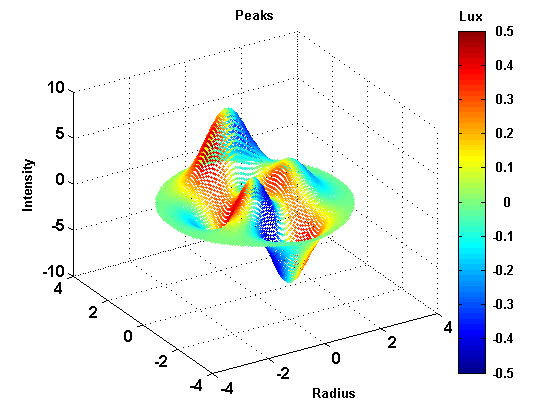
\includegraphics[width=.3\textwidth]{graf4d.png}
\caption{Exemplu graf 4d}\label{fig:logo}
\index{figures}
\end{figure}
%make-it sound better
Utilizând gradientul de culoare suntem capabili să vizualizăm o a patra dimensiune. 
\section{Ce este o hipersferă?}
În geometria dimensiunilor superioare, o hipersferă este ansamblul de puncte care se află la o distanță constantă fața de un punct dat numit centrul său.
Când o sferă are raza unității, este obișnuit să o numim unitate n-sferă sau pur și simplu n-sferă \cite{n-spheres}. În ceea ce privește norma standard, n-sfera este definită ca:\
\[
\S^{n}=\left\{x\in \mathbb {R} ^{n+1}:\left\|x\right\|=1\right\}
\]
Iar raza unei n-sfere este definită astfel:
\[
{\displaystyle S^{n}(r)=\left\{x\in \mathbb {R} ^{n+1}:\left\|x\right\|=r\right\}.}
\]
Dimensiunea n-sferei este n și \textbf{nu} trebuie confundată cu dimensiunea (n+1) a spațiului Euclidian în care este încorporată în mod natural. O n-sferă este suprafața, sau se alfla la limita unei bile in (n+1) dimensiuni.


%Exemple
%Perechea de puncte de la capetele unui segment de linie 
%(unidimensional) este o sferă 0
%Un cerc, care are circumferința unidimensională a unui disc 
%(bidimensional), este o sferă 1,
%Suprafața bidimensională a unei bile tridimensionale este o 2-sferă, %adesea numită pur și simplu sferă,
%Granița tridimensională a unei bile (cu patru dimensiuni) 4 este o 
%3-sferă,
%Granița n - 1 dimensională a unei bile (n-dimensionale) n este o sferă %(n - 1).


\chapter{Aria cercului}
\begin{equation}
\mathbb{
\section{Cum am demonstrat?}
Considerand cercul cu \(x^2+y^2= \mathbb  {R}^2\), jumatatea de sus, dar si cea de jos pot fi in mod explicit exprimate prin \(y=\pm \sqrt{\mathbb{R}^2-x^2}\), x fiind cuprins intre \mathbb{-R} si \mathbb{+R}, aria in cauza este data de integrala:
}
\end{equation}
\begin{equation}
\mathbb{
\begin{aligned}
\begin{array}{l}
\int_{-R}^{R} \int_{-\sqrt{R^{2}-x^{2}}}^{\sqrt{R^{2}-x^{2}}} d y d x\\
\end{array}
\end{aligned}
}
\end{equation}

\begin{figure}[hbt!]
\centering
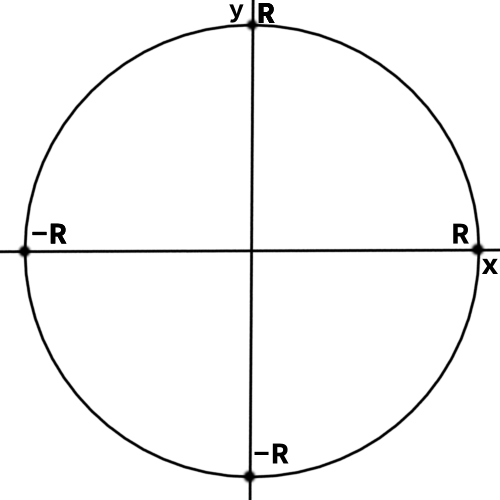
\includegraphics[width=.3\textwidth]{xoy_circle.png}
\caption{Sectiune cerc }\label{fig:logo}
\index{figures}
\end{figure}



\text {Prima integrala fiind calculata astfel:  }\\

\mathbb{
$$
\left.\int_{-R}^{R} y\right|_{-\sqrt{R^{2}-x^{2}}} ^{\sqrt{R^{2}-x^{2}}} d x &=\int_{-R}^{R} 2 \sqrt{R^{2}-x^{2}} d x \\
&=2 \int_{-R}^{R} \sqrt{R^{2}-x^{2}} d x
$$

\newpage{}
\section{Substituție trigonometrică}
Pentru a calcula $\int_{-R}^{R} \sqrt{R^{2}-x^{2}} d x$ folosim substitutia  trigonometrica $x=R \sin u$, rezultand ca $d x=R \cos u d u$.\\

$$
\begin{array}{l}
\text {Stiind ca} \cos \alpha \cos \beta=\frac{1}{2}(\cos (\alpha-\beta)+\cos (\alpha+\beta)), \text { avem }\cos ^{2} u=\frac{1}{2}(1+\cos 2 u) \\ \text { }
\end{array}
$$
}

\section{Demonstrație}

Dupa subistitutie rezulta urmatoare integrala:
$$
\begin{aligned}
\int R^{2} \cos ^{2} u d u &=R^{2} \int \cos ^{2} u d u \\
&=R^{2} \int \frac{1}{2}(1+\cos 2 u) d u \\
&=\frac{1}{2} R^{2}\left(u+\frac{1}{2} \sin 2 u\right)+A \\
&=\frac{1}{2} R^{2}(u+\sin u \cos u)+A
\end{aligned}
$$

$$
\begin{array}{l}
\text { Avand in vedere ca } x=R \sin u, \text { substituim } u=\sin ^{-1}(x / R) \text { pentru  ajunge la  }\\
\frac{1}{2} R^{2} \sin ^{-1}(x / R)+\frac{1}{2} x \sqrt{R^{2}-x^{2}}+A. \\ \text { Aplicand limitele de integrare } x \text { }
\text { de la }-R \text { pana } R, \text { deducem  urmatoarea formula  }\\ \left.\left[\frac{1}{2} R^{2} \sin ^{-1}(x / R)+\frac{1}{2} x \sqrt{R^{2}-x^{2}}\right]\right|_{-R} ^{R}=\frac{1}{2} \pi R^{2} \text { , }
\text { deoarece } \sin ^{-1}(\pm 1)=\pm \pi / 2 \text { . }
\end{array}
$$

\section{Concluzie}
 
\text{Prin argumentele prezentate mai sus, acestea concluzioneaza formula ariei:}
$$
\left.\int_{-R}^{R} y\right|_{-\sqrt{R^{2}-x^{2}}} ^{\sqrt{R^{2}-x^{2}}} d x=2 \int_{-R}^{R} \sqrt{R^{2}-x^{2}} d x=\pi R^{2} .
$$


\chapter{Volumul sferei}

\section{Ecuația sferei}

Ecuația pentru marginea exterioară a unei sfere cu raza r este dată de: $$ x^2 + y^2 + z^2 = r^2 $$ 
Dacă dorim să considerăm volumul din interiorul unei sfere, atunci trebuie să considerăm regiunea dată de inecuația \cite{university-of-washington-2013}:  $$x^2+y^2+z^2 \leq r^2 $$

\section{Coordonate sferice}

Utilizarea coordonatelor sferice este avantajoasă, astfel vom trece de la coordonate carteziene la sferice cu următoarea mapare \cite{spherical-coordinates}:

\begin{figure}[hbt!]
\centering
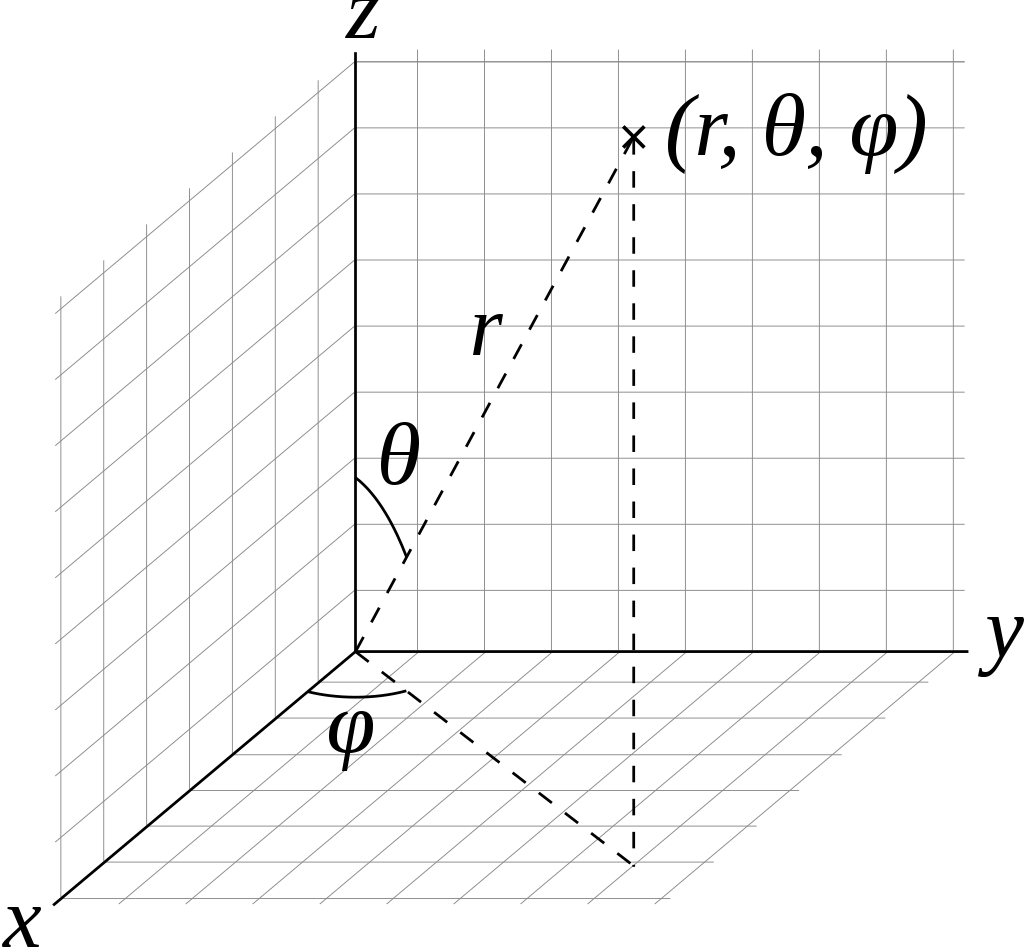
\includegraphics[width=.3\textwidth]{punct_coordonate_sferice.png}
\caption{Coordonate sferice în plan}\label{fig:logo}
\index{figures}
\end{figure}

In coordonate sferice, sfera reprezintă totalitatea punctelor unde aceste inecuații sunt satisfăcute:
$$
\begin{cases}
0 \leq \theta \leq \pi \\
0 \leq \phi \leq 2\pi \\
0 \leq \rho \leq r
\end{cases}
$$

Demonstrația se bazează pe integrala multiplă de determinare a volumului unui paralelipiped:

$$
\begin{aligned}
\iiint_{paralelipiped} 1 d V
&=\int_{a}^{b} \int_{c}^{d} \int_{p}^{q} 1 d z d y d x \\
&=(b-a)(d-c)(q-p)
\end{aligned}
$$


\section{Matricea Jacobiana si elementul de volum}

În spațiul Euclidian, elementul de volum este dat de produsul diferențialelor coordonatelor carteziene \cite{volume-element}.

$$
d V=d x d y d z
$$

În alte sisteme de coordonate, cum ar fi cele sferice, elementul de volum se schimbă in funcție de matricea Jacobiană a schimbării de coordonate \cite{jacobian-matrix}.

$$
d V=\left|\frac{\partial(x, y, z)}{\partial\left(u_{1}, u_{2}, u_{3}\right)}\right| d u_{1} d u_{2} d u_{3}
$$

Astfel matricea Jacobiană pentru sistemul de coordonate este:

$$
\begin{array}{l}
x=\rho \sin \varphi \cos \theta \\
y=\rho \sin \varphi \sin \theta \\
z=\rho \cos \varphi
\end{array}
$$

$$
\mathbf{J}_{\mathbf{F}}(\rho, \varphi, \theta)=\left[\begin{array}{lll}
\frac{\partial x}{\partial \rho} & \frac{\partial x}{\partial \varphi} & \frac{\partial x}{\partial \theta} \\
\frac{\partial y}{\partial \rho} & \frac{\partial y}{\partial \varphi} & \frac{\partial y}{\partial \theta} \\
\frac{\partial z}{\partial \rho} & \frac{\partial z}{\partial \varphi} & \frac{\partial z}{\partial \theta}
\end{array}\right]=\left[\begin{array}{ccc}
\sin \varphi \cos \theta & \rho \cos \varphi \cos \theta & -\rho \sin \varphi \sin \theta \\
\sin \varphi \sin \theta & \rho \cos \varphi \sin \theta & \rho \sin \varphi \cos \theta \\
\cos \varphi & -\rho \sin \varphi & 0
\end{array}\right]
$$

Calculând determinantul, și introducând în formulă pentru elementul de volum ne va genera:

$$
d V=\rho^{2} \sin \phi d \rho d \theta d \phi
$$

\section{Volumul sferei}

Astfel, trecând la coordonate sferice, și schimbând limitele integralelor la limitele unei sfere, putem afla volumul unei sfere prin integrarea elementului de volum:

$$
\begin{aligned}
\iiint_{sfera} 1 d V
&=\int_{0}^{\pi} \int_{0}^{2 \pi} \int_{0}^{r} \rho^{2} \sin (\theta) d \rho d \phi d \theta \\
&=\int_{0}^{\pi} \sin (\theta) d \theta \int_{0}^{2 \pi} d \phi \int_{0}^{r} \rho^{2} d \rho \\
&=(2)(2 \pi)\left(\frac{1}{3} r^{3}\right) \\
&=\frac{4}{3} \pi r^{3}
\end{aligned}
$$



Astfel, volumul sferei se poate calcula utilizând o integrală multiplă, în trei dimensiuni, iar formula generală este:

$$
V_3 = \frac{4\pi R^3}{3}
$$


\chapter{Volumul hipersferei in 4 dimensiuni}

\section{Demonstrație}

Demonstrația de la volumul sferei se poate extinde în mai multe dimensiuni, generând astfel coordonate sferice în patru dimensiuni.

\section{Coordonate sferice}

Unghiurile care trebuie considerate în patru dimensiuni sunt următoarele:
$$
\begin{cases}
0 \leq \theta \leq \pi \\
0 \leq \phi \leq 2\pi \\
0 \leq \rho \leq r \\
0 \leq \Phi \leq 2\pi
\end{cases}
$$

\section{Matricea Jacobiana si elementul de volum}

Matricea Jacobiană va fi generată de următorul sistem:

$$
\begin{array}{l}
x=\rho \sin \varphi \cos \theta \\
y=\rho \sin \varphi \sin \theta \sin \Phi \\
z=\rho \sin \varphi \sin \theta \sin \phi \\
w=\rho \cos \varphi
\end{array}
$$

\begin{figure}[hbt!]
\centering
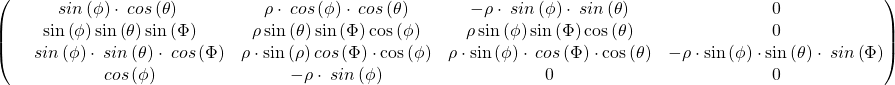
\includegraphics[width=1\textwidth]{determinant.png}
\caption{Determinant Jacobian}\label{fig:logo}
\index{figures}
\end{figure}

Astfel, rezolvând determinantul, elementul de volum generat va fi:

$$
d V=\rho^3\sin ^2\left(\phi\right)\sin ^2\left(\Phi\right)\sin \left(\theta\right)
$$

\section{Volumul hipersferei}

Introducând elementul de volum în integrala multidimensională, ne va genera urmatoarea:

$$
\begin{aligned}
\iiiint_{hipersfera} 1 d V= \\ 
&=\int _0^{2\pi }\int _0^{\pi }\int _0^{2\pi }\int _0^r\rho^3\sin ^2\left(\phi\right)\sin \left(\theta\right)\cos ^2\left(\Phi\right)d\rho\d\phi d\theta d\Phi \\
&=\int _0^{2\pi }\int _0^{\pi }\int _0^{2\pi }\sin ^2\left(\phi\right)\cos ^2\left(\Phi\right)\sin \left(\theta\right)\frac{r^4}{4}d\phi Volumul hipersferelord\theta d\Phi \\
&=\int _0^{2\pi }\int _0^{\pi }\frac{\pi r^4\cos ^2\left(\Phi\right)}{4}\sin \left(\theta\right)d\theta d\Phi \\
&=\int _0^{2\pi }\left(\frac{\pi r^4\cos ^2\left(\Phi\right)}{2}\right)d\Phi \\
&=\frac{\pi ^2r^4}{2}
\end{aligned}
$$

Astfel, volumul sferei se poate calcula utilizând o integrală multiplă, în patru dimensiuni, iar formula generală este:

$$
V_4 = \frac{\pi ^2r^4}{2}
$$

\chapter{Volumul n-sferei}
\section{Integrare si utilizare coordonatelor sferice}
Volumul poate fi calculat prin integrarea elementului de volum în coordonate sferice. \\
Sistem de coordonate sferice poseda o coordonata radiala ‚r, dar si o coordonata unghiulara \(\phi\)1,…, \(\phi\)n - 1, unde domeniul fiecărui\(\phi\), cu excepția \(\phi\)n – 1, il reprezinta [0, \(\pi\)), iar domeniul \(\phi\)n - 1 este [0, 2\(\pi\)) . Elementul de volum sferic este precizat in urmatoatea formula:



$$
d V=r^{n-1} \sin ^{n-2}\left(\varphi_{1}\right) \sin ^{n-3}\left(\varphi_{2}\right) \cdots \sin \left(\varphi_{n-2}\right) d r d \varphi_{1} d \varphi_{2} \cdots d \varphi_{n-1},
$$
Iar volumul este integrala acestei mărimi cu r între 0 și \mathbb{R}, de asemenea și toate unghiurile posibile:
$$
V_{n}(R)=\int_{0}^{R} \int_{0}^{\pi} \cdots \int_{0}^{2 \pi} r^{n-1} \sin ^{n-2}\left(\varphi_{1}\right) \cdots \sin \left(\varphi_{n-2}\right) d \varphi_{n-1} \cdots d \varphi_{1} d r .
$$
Fiecare dintre factori depinde doar de o singură variabilă și, prin urmare, integrala iterată poate fi scrisă ca produs al integralelor:

$$
V_{n}(R)=\left(\int_{0}^{R} r^{n-1} d r\right)\left(\int_{0}^{\pi} \sin ^{n-2}\left(\varphi_{1}\right) d \varphi_{1}\right) \cdots\left(\int_{0}^{2 \pi} d \varphi_{n-1}\right)
$$


Luand in considerare faptul ca integrala cu raza este Rn/n si intervalele de integrare pe coordonatele
unghiulare pot fi calculate simetric, schimbandu-se in [0, \(\pi\)/2]:


$$
V_{n}(R)=\frac{R^{n}}{n}\left(2 \int_{0}^{\frac{\pi}{2}} \sin ^{n-2}\left(\varphi_{1}\right) d \varphi_{1}\right) \cdots\left(4 \int_{0}^{\frac{\pi}{2}} d \varphi_{n-1}\right) .
$$
Fiecare integrala care a ramas reprezinta o anumita valoare speciala pentru functia beta:
\section{Ce este functia Beta ?}
În matematică, funcția beta, numită și integrala Euler, este o funcție specială, care este strânsa legată de funcția Gamma și de coeficienții binomiali. Este definit de integrala
$$
\mathrm{B}(x, y)=\int_{0}^{1} t^{x-1}(1-t)^{y-1} d t
$$
O scurta reprezentare grafica a functie Beta

\begin{figure}[hbt!]
\centering
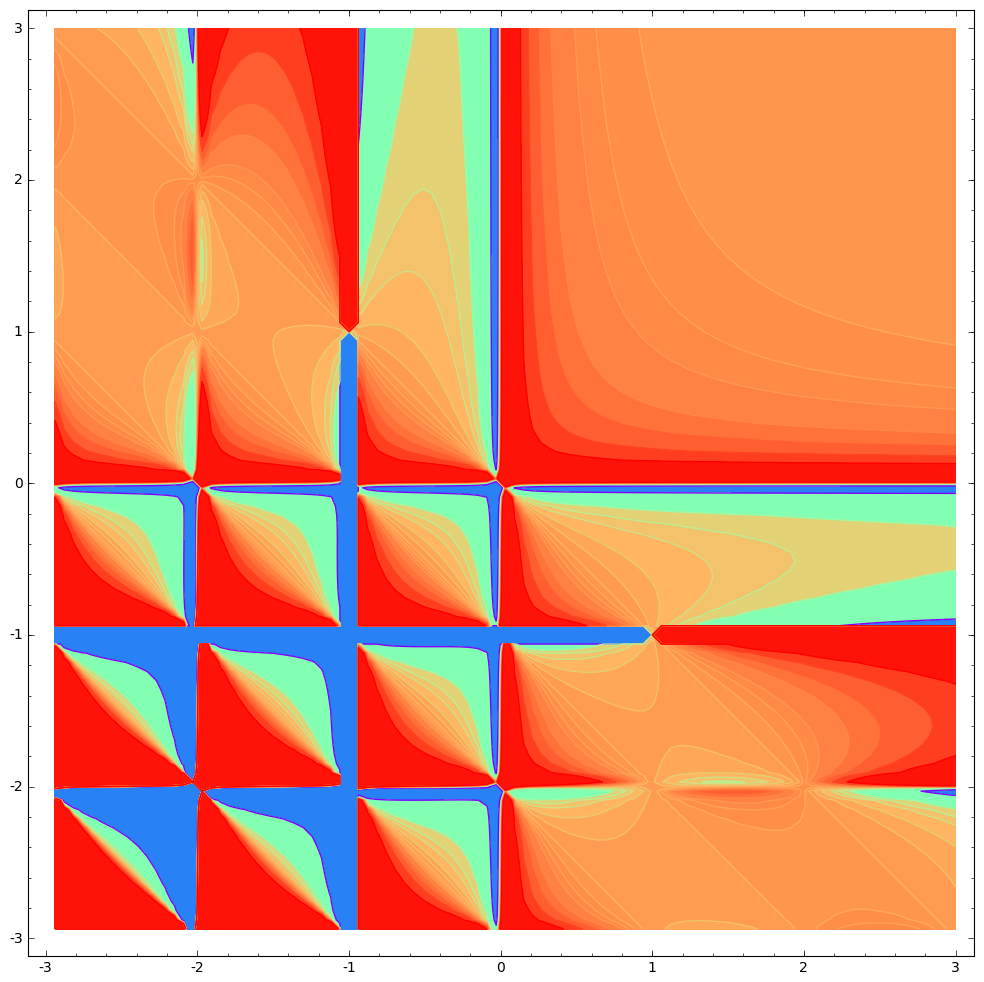
\includegraphics[width=.5\textwidth]{beta.png}
\caption{Functie Beta}\label{fig:logo}
\index{figures}
\end{figure}

$$
V_{n}(R)=\frac{R^{n}}{n} \mathrm{~B}\left(\frac{n-1}{2}, \frac{1}{2}\right) \mathrm{B}\left(\frac{n-2}{2}, \frac{1}{2}\right) \cdots \mathrm{B}\left(1, \frac{1}{2}\right) \cdot 2 \mathrm{~B}\left(\frac{1}{2}, \frac{1}{2}\right) .
$$

Functiile beta pot fi rescrise in termini de functii gamma:

\section{Ce este o functie Gamma ?}
In matematica, functia gamma (reprezentata de  \(\Gamma\), litera mare gamma din alfabetul grecesc) este una dintre cele mai utilizate metode de a reprezenta functia factorial pentru numere complexe dar nu numai. Functia gamma este definita pentru toate numerele complexe excluzand numerele negative. Pentru orice numar poziv gamma de n este egal cu:
\[\Gamma(n) = (n-1)!\]
Exista cateva conventii pentru Gamma:
$$
\Gamma\left(\frac{1}{2}\right)=\sqrt{\pi} 
$$
$$
\Gamma(0)=1
$$

Acesta proprietate care ne spune ca \(\Gamma\) de 1/2 are o valoare ne ajuta sa calculam Gamma pentru orice alt numar fractionar.
Si daca dorim sa calculam Gamma putem folosi una dintre cele doua variante care implica Functia beta explicata mai sus:


$$
\begin{array}{l}
\Gamma\left(\frac{1}{2}+n\right)=\frac{(2 n) !}{4^{n} n !} \sqrt{\pi}=\frac{(2 n-1) ! !}{2^{n}} \sqrt{\pi}=\left(\begin{array}{c}
n-\frac{1}{2} \\
n
\end{array}\right) n ! \sqrt{\pi} \\
\Gamma\left(\frac{1}{2}-n\right)=\frac{(-4)^{n} n !}{(2 n) !} \sqrt{\pi}=\frac{(-2)^{n}}{(2 n-1) ! !} \sqrt{\pi}=\frac{\sqrt{\pi}}{(-1 / 2) n !}
\end{array}
$$

\section{Relatia dintre Functia Gamma si Functia Beta}

Ca sa putem urmatoarea cerinta trebuie sa rescriem relatie dintre cele doua functii Gamma ca un produs de functii exponentiale
$$
\mathrm{B}(x, y)=\frac{\Gamma(x) \Gamma(y)}{\Gamma(x+y)}
$$

reszultand:
$$
\begin{aligned}
\Gamma(x) \Gamma(y) &=\int_{u=0}^{\infty} e^{-u} u^{x-1} d u \cdot \int_{v=0}^{\infty} e^{-v} v^{y-1} d v \\
&=\int_{v=0}^{\infty} \int_{u=0}^{\infty} e^{-u-v} u^{x-1} v^{y-1} d u d v
\end{aligned}
$$
Schimband valoarea cu u = zt si v = z(1 − t) produce urmatoarele schimbari:

$$
\begin{aligned}
\Gamma(x) \Gamma(y) &=\int_{z=0}^{\infty} \int_{t=0}^{1} e^{-z}(z t)^{x-1}(z(1-t))^{y-1} z d t d z \\
&=\int_{z=0}^{\infty} e^{-z} z^{x+y-1} d z \cdot \int_{t=0}^{1} t^{x-1}(1-t)^{y-1} d t \\
&=\Gamma(x+y) \cdot \mathrm{B}(x, y) .
\end{aligned}
$$
Simplificand in ambele parti cu \(\Gamma(x+y)\) obtineme rezultatul dorit.
Identitatea declarată poate fi văzută ca un caz particular al identității pentru integrala unei convoluții. 
\section{Integrale convolutive}
Dacă f și g sunt funcții integrabile, atunci integralul convoluției lor pe întreg spațiul se obține pur și simplu ca produs al integralelor lor:
$$
\int_{\mathbf{R}^{d}}(f * g)(x) d x=\left(\int_{\mathbf{R}^{d}} f(x) d x\right)\left(\int_{\mathbf{R}^{d}} g(x) d x\right)
$$
Aceasta integrala utilizieaza Teorema lui  Fubini's:
În analiza matematică, teorema lui Fubini, introdusă de Guido Fubini în 1907, este un rezultat care oferă condiții în care este posibil să se calculeze o integrală dublă utilizând o integrală iterată. Se poate schimba ordinea integrării dacă integrala dublă dă un răspuns finit atunci când integrandul este înlocuit cu valoarea sa absolută.
$$
\int_{X \times Y} f(x, y) \mathrm{d}(x, y)=\int_{X}\left(\int_{Y} f(x, y) \mathrm{d} y\right) \mathrm{d} x=\int_{Y}\left(\int_{X} f(x, y) \mathrm{d} x\right) \mathrm{d} y
$$



Luând:
$$
\begin{array}{l}
f(u):=e^{-u} u^{x-1} 1_{\mathbb{R}_{+}} \\
g(u):=e^{-u} u^{y-1} 1_{\mathbb{R}_{+}}
\end{array}
$$
avand ca:
$$
\Gamma(x) \Gamma(y)=\int_{\mathbb{R}} f(u) d u \cdot \int_{\mathbb{R}} g(u) d u=\int_{\mathbb{R}}(f * g)(u) d u=\mathrm{B}(x, y) \Gamma(x+y) .
$$



\section{Demonstratie}
Utilizand subistitutiile enuntate mai sus obtine in cele din urma:
$$
V_{n}(R)=\frac{R^{n}}{n} \frac{\Gamma\left(\frac{n-1}{2}\right) \Gamma\left(\frac{1}{2}\right)}{\Gamma\left(\frac{n}{2}\right)} \frac{\Gamma\left(\frac{n-2}{2}\right) \Gamma\left(\frac{1}{2}\right)}{\Gamma\left(\frac{n-1}{2}\right)} \cdots \frac{\Gamma(1) \Gamma\left(\frac{1}{2}\right)}{\Gamma\left(\frac{3}{2}\right)} \cdot 2 \frac{\Gamma\left(\frac{1}{2}\right) \Gamma\left(\frac{1}{2}\right)}{\Gamma(1)}
$$
Prin urmare, combinand formula de mai sus cu valorile \(\Gamma\) (1/2) = \(\sqrt{ \pi }\)  și  \(\Gamma\) (1) = 1, dar și ecuația funcțională z \(\Gamma\) (z) = \(\Gamma\) (z + 1) rezulta:
$$
V_{n}(R)=\frac{2 \pi^{\frac{n}{2}} R^{n}}{n \Gamma\left(\frac{n}{2}\right)}=\frac{\pi^{\frac{n}{2}} R^{n}}{\Gamma\left(\frac{n}{2}+1\right)}
$$




\newpage
\chapter{Curiozitati}
\text


Dupa o scurta analiza putem oberva ca nici suprafata nu creste exponential la in functie de cum adaugam n dimensiune. In graficul de mai jos ne este ilustrata scaling in ariei si volumului in functie de numarul de dimensiuni.

\begin{figure}[hbt!]
\centering
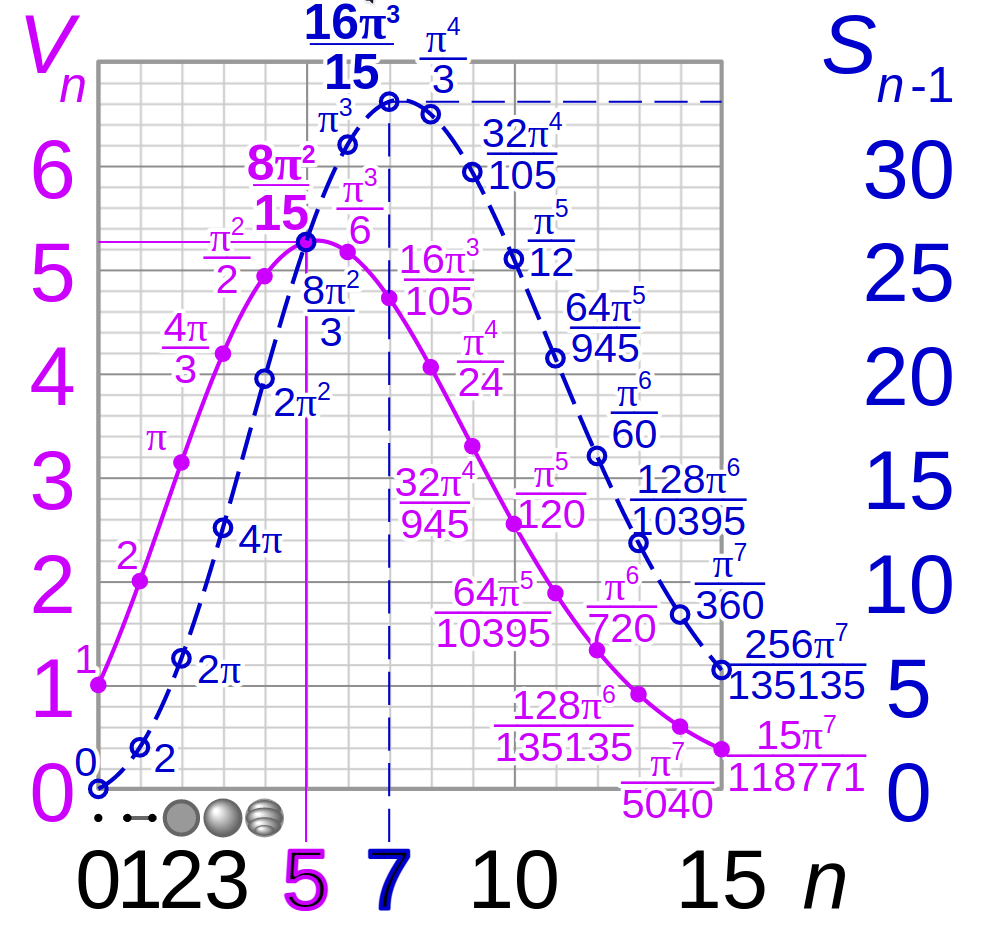
\includegraphics[width=.9\textwidth]{rap_arrii.png}
\caption{Raport arii si volum}\label{fig:logo}
\index{figures}
\end{figure}

\newpage
Aici avem o mica schema care ne exemplifica volumul si aria in n dimensiuni:

\begin{figure}[hbt!]
\centering
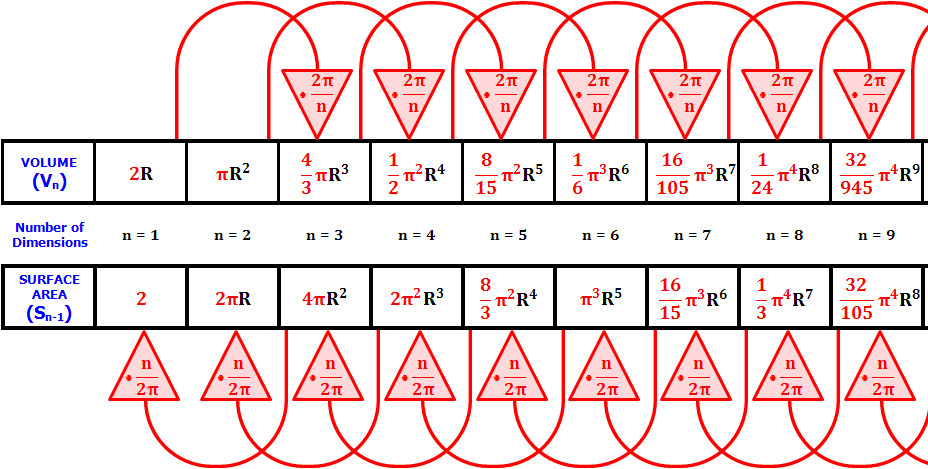
\includegraphics[width=1\textwidth]{volume_area.png}
\caption{Raport arii si volum}\label{fig:logo}
\index{figures}
\end{figure}



\printbibliography


%\appendix
%\printindex
%\theendnotes

\end{document}
